% Options for packages loaded elsewhere
\PassOptionsToPackage{unicode}{hyperref}
\PassOptionsToPackage{hyphens}{url}
%
\documentclass[
]{article}
\usepackage{amsmath,amssymb}
\usepackage{lmodern}
\usepackage{iftex}
\ifPDFTeX
  \usepackage[T1]{fontenc}
  \usepackage[utf8]{inputenc}
  \usepackage{textcomp} % provide euro and other symbols
\else % if luatex or xetex
  \usepackage{unicode-math}
  \defaultfontfeatures{Scale=MatchLowercase}
  \defaultfontfeatures[\rmfamily]{Ligatures=TeX,Scale=1}
\fi
% Use upquote if available, for straight quotes in verbatim environments
\IfFileExists{upquote.sty}{\usepackage{upquote}}{}
\IfFileExists{microtype.sty}{% use microtype if available
  \usepackage[]{microtype}
  \UseMicrotypeSet[protrusion]{basicmath} % disable protrusion for tt fonts
}{}
\makeatletter
\@ifundefined{KOMAClassName}{% if non-KOMA class
  \IfFileExists{parskip.sty}{%
    \usepackage{parskip}
  }{% else
    \setlength{\parindent}{0pt}
    \setlength{\parskip}{6pt plus 2pt minus 1pt}}
}{% if KOMA class
  \KOMAoptions{parskip=half}}
\makeatother
\usepackage{xcolor}
\usepackage[margin=1in]{geometry}
\usepackage{color}
\usepackage{fancyvrb}
\newcommand{\VerbBar}{|}
\newcommand{\VERB}{\Verb[commandchars=\\\{\}]}
\DefineVerbatimEnvironment{Highlighting}{Verbatim}{commandchars=\\\{\}}
% Add ',fontsize=\small' for more characters per line
\usepackage{framed}
\definecolor{shadecolor}{RGB}{248,248,248}
\newenvironment{Shaded}{\begin{snugshade}}{\end{snugshade}}
\newcommand{\AlertTok}[1]{\textcolor[rgb]{0.94,0.16,0.16}{#1}}
\newcommand{\AnnotationTok}[1]{\textcolor[rgb]{0.56,0.35,0.01}{\textbf{\textit{#1}}}}
\newcommand{\AttributeTok}[1]{\textcolor[rgb]{0.77,0.63,0.00}{#1}}
\newcommand{\BaseNTok}[1]{\textcolor[rgb]{0.00,0.00,0.81}{#1}}
\newcommand{\BuiltInTok}[1]{#1}
\newcommand{\CharTok}[1]{\textcolor[rgb]{0.31,0.60,0.02}{#1}}
\newcommand{\CommentTok}[1]{\textcolor[rgb]{0.56,0.35,0.01}{\textit{#1}}}
\newcommand{\CommentVarTok}[1]{\textcolor[rgb]{0.56,0.35,0.01}{\textbf{\textit{#1}}}}
\newcommand{\ConstantTok}[1]{\textcolor[rgb]{0.00,0.00,0.00}{#1}}
\newcommand{\ControlFlowTok}[1]{\textcolor[rgb]{0.13,0.29,0.53}{\textbf{#1}}}
\newcommand{\DataTypeTok}[1]{\textcolor[rgb]{0.13,0.29,0.53}{#1}}
\newcommand{\DecValTok}[1]{\textcolor[rgb]{0.00,0.00,0.81}{#1}}
\newcommand{\DocumentationTok}[1]{\textcolor[rgb]{0.56,0.35,0.01}{\textbf{\textit{#1}}}}
\newcommand{\ErrorTok}[1]{\textcolor[rgb]{0.64,0.00,0.00}{\textbf{#1}}}
\newcommand{\ExtensionTok}[1]{#1}
\newcommand{\FloatTok}[1]{\textcolor[rgb]{0.00,0.00,0.81}{#1}}
\newcommand{\FunctionTok}[1]{\textcolor[rgb]{0.00,0.00,0.00}{#1}}
\newcommand{\ImportTok}[1]{#1}
\newcommand{\InformationTok}[1]{\textcolor[rgb]{0.56,0.35,0.01}{\textbf{\textit{#1}}}}
\newcommand{\KeywordTok}[1]{\textcolor[rgb]{0.13,0.29,0.53}{\textbf{#1}}}
\newcommand{\NormalTok}[1]{#1}
\newcommand{\OperatorTok}[1]{\textcolor[rgb]{0.81,0.36,0.00}{\textbf{#1}}}
\newcommand{\OtherTok}[1]{\textcolor[rgb]{0.56,0.35,0.01}{#1}}
\newcommand{\PreprocessorTok}[1]{\textcolor[rgb]{0.56,0.35,0.01}{\textit{#1}}}
\newcommand{\RegionMarkerTok}[1]{#1}
\newcommand{\SpecialCharTok}[1]{\textcolor[rgb]{0.00,0.00,0.00}{#1}}
\newcommand{\SpecialStringTok}[1]{\textcolor[rgb]{0.31,0.60,0.02}{#1}}
\newcommand{\StringTok}[1]{\textcolor[rgb]{0.31,0.60,0.02}{#1}}
\newcommand{\VariableTok}[1]{\textcolor[rgb]{0.00,0.00,0.00}{#1}}
\newcommand{\VerbatimStringTok}[1]{\textcolor[rgb]{0.31,0.60,0.02}{#1}}
\newcommand{\WarningTok}[1]{\textcolor[rgb]{0.56,0.35,0.01}{\textbf{\textit{#1}}}}
\usepackage{longtable,booktabs,array}
\usepackage{calc} % for calculating minipage widths
% Correct order of tables after \paragraph or \subparagraph
\usepackage{etoolbox}
\makeatletter
\patchcmd\longtable{\par}{\if@noskipsec\mbox{}\fi\par}{}{}
\makeatother
% Allow footnotes in longtable head/foot
\IfFileExists{footnotehyper.sty}{\usepackage{footnotehyper}}{\usepackage{footnote}}
\makesavenoteenv{longtable}
\usepackage{graphicx}
\makeatletter
\def\maxwidth{\ifdim\Gin@nat@width>\linewidth\linewidth\else\Gin@nat@width\fi}
\def\maxheight{\ifdim\Gin@nat@height>\textheight\textheight\else\Gin@nat@height\fi}
\makeatother
% Scale images if necessary, so that they will not overflow the page
% margins by default, and it is still possible to overwrite the defaults
% using explicit options in \includegraphics[width, height, ...]{}
\setkeys{Gin}{width=\maxwidth,height=\maxheight,keepaspectratio}
% Set default figure placement to htbp
\makeatletter
\def\fps@figure{htbp}
\makeatother
\setlength{\emergencystretch}{3em} % prevent overfull lines
\providecommand{\tightlist}{%
  \setlength{\itemsep}{0pt}\setlength{\parskip}{0pt}}
\setcounter{secnumdepth}{5}
\usepackage{booktabs}
\ifLuaTeX
  \usepackage{selnolig}  % disable illegal ligatures
\fi
\usepackage[]{natbib}
\bibliographystyle{apalike}
\IfFileExists{bookmark.sty}{\usepackage{bookmark}}{\usepackage{hyperref}}
\IfFileExists{xurl.sty}{\usepackage{xurl}}{} % add URL line breaks if available
\urlstyle{same} % disable monospaced font for URLs
\hypersetup{
  pdftitle={gapclosing: An R package},
  pdfauthor={Ian Lundberg (ilundberg@cornell.edu)},
  hidelinks,
  pdfcreator={LaTeX via pandoc}}

\title{gapclosing: An R package}
\author{Ian Lundberg (\href{mailto:ilundberg@cornell.edu}{\nolinkurl{ilundberg@cornell.edu}})}
\date{2023-03-08}

\begin{document}
\maketitle

{
\setcounter{tocdepth}{2}
\tableofcontents
}
\hypertarget{gapclosing-an-r-package}{%
\section{gapclosing: An R package}\label{gapclosing-an-r-package}}

To what degree would a hypothetical intervention close gaps across populations?

This causal question is of paramount importance for those who want to intervene to reduce disparities across categories such as gender, race, and class. How to answer that question is the subject of the companion papaer to this package.

\begin{quote}
Lundberg, Ian. 2022. \href{https://doi.org/10.1177/00491241211055769}{``The gap-closing estimand: A causal approach to study interventions that close disparities across social categories.''} \emph{Sociological Methods and Research}.
\end{quote}

To get started with these methods, first install \href{https://rstudio-education.github.io/hopr/starting.html}{R and RStudio}. Then install the package from CRAN.

\begin{Shaded}
\begin{Highlighting}[]
\FunctionTok{install.packages}\NormalTok{(}\StringTok{"gapclosing"}\NormalTok{)}
\end{Highlighting}
\end{Shaded}

You can now do lots of things!

\begin{itemize}
\tightlist
\item
  Estimate treatment and outcome prediction functions statistical and machine learning methods
\item
  Combine those in doubly-robust estimators of gap-closing estimands
\item
  Produce confidence intervals by the bootstrap
\item
  Visualize the result
\end{itemize}

Questions and comments to Ian Lundberg, \href{mailto:ilundberg@cornell.edu}{\nolinkurl{ilundberg@cornell.edu}}.

\hypertarget{big-idea}{%
\section{Big idea}\label{big-idea}}

This part introduces the big ideas: why we should do this, what data look like, and what's going on under the hood. It closes with basic package functionality.

\hypertarget{motivation}{%
\subsection{Motivation}\label{motivation}}

Gaps across social categories like race, class, and gender are important to understand. We would like to know whether there is anything we can do to close these gaps. What if we intervened to reduce incarceration or increase access to education? Would those interventions close gaps across categories of race, class, or gender?

These types of questions are at the core of a growing literature in epidemiology addresses these questions with techniques for causal decomposition analysis (\citet{vanderweele2014}, \citet{jackson2018}, \citet{jackson2020}). The paper which accompanies this software package introduces these methods to a broader set of social scientists.

\begin{quote}
Lundberg, Ian. 2022. ``The gap-closing estimand: A causal approach to study interventions that close disparities across social categories.'' \emph{Sociological Methods and Research}. \href{https://doi.org/10.1177/00491241211055769}{{[}published version{]}} \href{https://doi.org/10.31235/osf.io/gx4y3}{{[}open access preprint{]}} \href{https://ilundberg.github.io/gapclosing/}{{[}software{]}}.
\end{quote}

This package provides software to support inquiry into gap-closing estimands. A guiding principle is to partition the tasks the human user must do from the tasks that the package can automate.

The human user must carry out these tasks:

\begin{itemize}
\tightlist
\item
  Define the intervention
\item
  Make causal assumptions for identification
\item
  Specify a treatment model and/or an outcome model
\end{itemize}

Given those inputs, the package will automatically:

\begin{itemize}
\tightlist
\item
  Estimate models (GLM, GAM, ridge regression, or random forest)
\item
  Convert models to doubly-robust estimates of gap-closing estimands, using sample splitting to improve convergence
\item
  Estimate standard errors by bootstrapping
\item
  Visualize the result
\end{itemize}

\hypertarget{data-structure}{%
\subsection{Data structure}\label{data-structure}}

In a data frame \texttt{data}, we have a gap-defining category such as race, gender, or class. We have a binary treatment variable that could have counterfactually been different for any individual. We want to know the degree to which an intervention to change the treatment would close gaps across the categories.

\begin{quote}
\textbf{These boxes will present an example.}

\emph{Example.} Suppose we have the following data.

\begin{itemize}
\tightlist
\item
  \(X\) (\texttt{category}): Category of interest, taking values \{A, B, C\}
\item
  \(T\) (\texttt{treatment}): Binary treatment variable, taking values 0 and 1
\item
  \(L\) (\texttt{confounder}): A continuous confounding variable, Uniform(-1,1)
\item
  \(Y\) (\texttt{outcome}): A continuous outcome variable, conditionally normal
\end{itemize}
\end{quote}

\begin{Shaded}
\begin{Highlighting}[]
\FunctionTok{set.seed}\NormalTok{(}\DecValTok{08544}\NormalTok{)}
\FunctionTok{library}\NormalTok{(gapclosing)}
\FunctionTok{library}\NormalTok{(dplyr)}
\FunctionTok{library}\NormalTok{(ggplot2)}
\end{Highlighting}
\end{Shaded}

\begin{Shaded}
\begin{Highlighting}[]
\NormalTok{simulated\_data }\OtherTok{\textless{}{-}} \FunctionTok{generate\_simulated\_data}\NormalTok{(}\AttributeTok{n =} \DecValTok{1000}\NormalTok{)}
\FunctionTok{head}\NormalTok{(simulated\_data)}
\CommentTok{\#\textgreater{}   category confounder treatment    outcome}
\CommentTok{\#\textgreater{} 1        C   1.640509         1 {-}0.7970377}
\CommentTok{\#\textgreater{} 2        B   1.032373         0  1.9304909}
\CommentTok{\#\textgreater{} 3        C   2.217630         1 {-}0.2009803}
\CommentTok{\#\textgreater{} 4        A  {-}1.642914         0 {-}0.5015702}
\CommentTok{\#\textgreater{} 5        A  {-}1.844897         0 {-}1.2027025}
\CommentTok{\#\textgreater{} 6        A  {-}2.415100         0 {-}3.9288188}
\end{Highlighting}
\end{Shaded}

\hypertarget{coding-from-scratch}{%
\subsection{Coding from scratch}\label{coding-from-scratch}}

With the most simple models, you can carry out a gap-closing analysis without the software package. First, fit any prediction function for the outcome as a function of the category of interest, confounders, and treatment.

\begin{Shaded}
\begin{Highlighting}[]
\NormalTok{example\_ols }\OtherTok{\textless{}{-}} \FunctionTok{lm}\NormalTok{(outcome }\SpecialCharTok{\textasciitilde{}}\NormalTok{ category}\SpecialCharTok{*}\NormalTok{treatment }\SpecialCharTok{+}\NormalTok{ confounder,}
                  \AttributeTok{data =}\NormalTok{ simulated\_data)}
\end{Highlighting}
\end{Shaded}

For everyone in the sample, predict under a counterfactual treatment value (e.g., \texttt{treatment\ =\ 1}).

\begin{Shaded}
\begin{Highlighting}[]
\NormalTok{fitted }\OtherTok{\textless{}{-}}\NormalTok{ simulated\_data }\SpecialCharTok{\%\textgreater{}\%}
  \FunctionTok{mutate}\NormalTok{(}\AttributeTok{outcome\_under\_treatment\_1 =} \FunctionTok{predict}\NormalTok{(example\_ols,}
                                             \AttributeTok{newdata =}\NormalTok{ simulated\_data }\SpecialCharTok{\%\textgreater{}\%}
                                               \FunctionTok{mutate}\NormalTok{(}\AttributeTok{treatment =} \DecValTok{1}\NormalTok{)))}
\end{Highlighting}
\end{Shaded}

Average the counterfactual estimates within each category.

\begin{Shaded}
\begin{Highlighting}[]
\NormalTok{fitted }\SpecialCharTok{\%\textgreater{}\%}
  \CommentTok{\# Group by the category of interest}
  \FunctionTok{group\_by}\NormalTok{(category) }\SpecialCharTok{\%\textgreater{}\%}
  \CommentTok{\# Take the average prediction}
  \FunctionTok{summarize}\NormalTok{(}\AttributeTok{factual =} \FunctionTok{mean}\NormalTok{(outcome),}
            \AttributeTok{counterfactual =} \FunctionTok{mean}\NormalTok{(outcome\_under\_treatment\_1))}
\CommentTok{\#\textgreater{} \# A tibble: 3 x 3}
\CommentTok{\#\textgreater{}   category factual counterfactual}
\CommentTok{\#\textgreater{}   \textless{}chr\textgreater{}      \textless{}dbl\textgreater{}          \textless{}dbl\textgreater{}}
\CommentTok{\#\textgreater{} 1 A        {-}1.09           0.0488}
\CommentTok{\#\textgreater{} 2 B        {-}0.0384        {-}0.0370}
\CommentTok{\#\textgreater{} 3 C         0.495          0.132}
\end{Highlighting}
\end{Shaded}

The software package supports these steps as well as more complex things you might want:

\begin{itemize}
\tightlist
\item
  three estimation strategies

  \begin{itemize}
  \tightlist
  \item
    outcome prediction
  \item
    treatment prediction
  \item
    doubly robust estimation
  \end{itemize}
\item
  machine learning prediction functions
\item
  counterfactual treatments that differ across units
\item
  bootstrapping for standard errors
\item
  easy visualization
\end{itemize}

\hypertarget{basic-package-functionality}{%
\subsection{Basic package functionality}\label{basic-package-functionality}}

The \texttt{gapclosing()} function estimates gaps across categories and the degree to which they would close under the specified \texttt{counterfactual\_assignments} of the treatment.

\begin{Shaded}
\begin{Highlighting}[]
\NormalTok{estimate }\OtherTok{\textless{}{-}} \FunctionTok{gapclosing}\NormalTok{(}
  \AttributeTok{data =}\NormalTok{ simulated\_data,}
  \AttributeTok{counterfactual\_assignments =} \DecValTok{1}\NormalTok{,}
  \AttributeTok{outcome\_formula =} \FunctionTok{formula}\NormalTok{(outcome }\SpecialCharTok{\textasciitilde{}}\NormalTok{ confounder }\SpecialCharTok{+}\NormalTok{ category}\SpecialCharTok{*}\NormalTok{treatment),}
  \AttributeTok{treatment\_formula =} \FunctionTok{formula}\NormalTok{(treatment }\SpecialCharTok{\textasciitilde{}}\NormalTok{ confounder }\SpecialCharTok{+}\NormalTok{ category),}
  \AttributeTok{category\_name =} \StringTok{"category"}\NormalTok{,}
  \AttributeTok{se =} \ConstantTok{TRUE}\NormalTok{,}
  \CommentTok{\# Setting bootstrap\_samples very low to speed this tutorial}
  \CommentTok{\# Should be set higher in practice}
  \AttributeTok{bootstrap\_samples =} \DecValTok{20}\NormalTok{,}
  \CommentTok{\# You can process the bootstrap in parallel with as many cores as available}
  \AttributeTok{parallel\_cores =} \DecValTok{1}
\NormalTok{)}
\end{Highlighting}
\end{Shaded}

By default, this function will do the following:

\begin{itemize}
\tightlist
\item
  Fit logistic regression to predict treatment assignment
\item
  Fit OLS regression to predict outcomes
\item
  Combine the two in a doubly-robust estimator estimated on a single sample
\item
  Return a \texttt{gapclosing} object which supports \texttt{summary}, \texttt{print}, and \texttt{plot} functions.
\end{itemize}

In this example, the \texttt{plot(estimate)} function produces the following visualization. The factual outcomes are unequal across categories, but the counterfactual outcomes are roughly equal. In this simulated setting, the intervention almost entirely closes the gaps across the categories.

\begin{Shaded}
\begin{Highlighting}[]
\FunctionTok{plot}\NormalTok{(estimate)}
\end{Highlighting}
\end{Shaded}

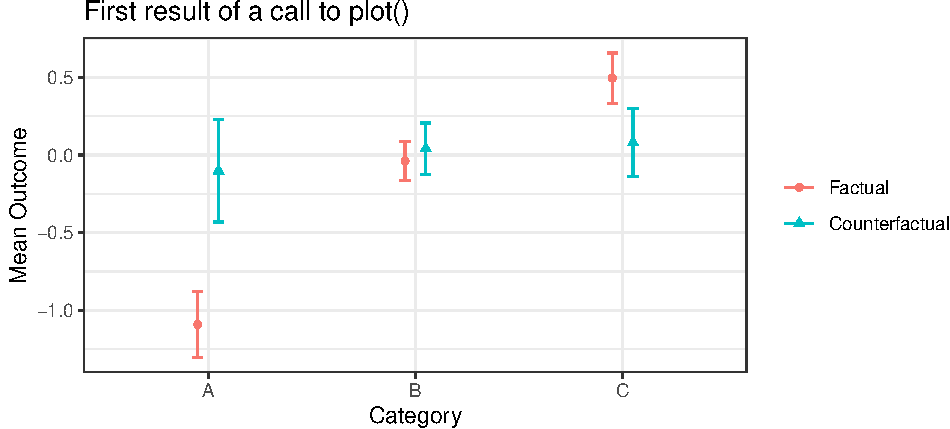
\includegraphics{github_doc_files/figure-latex/unnamed-chunk-12-1.pdf}

The \texttt{disparityplot()} function lets us zoom in on the factual and counterfactual disparity between two categories, of interest. In this case, we see that the intervention lifts outcomes in category A to be more comparable to category B. A \texttt{disparityplot} is a \texttt{ggplot2} object and can be customized by passing additional layers.

\begin{Shaded}
\begin{Highlighting}[]
\FunctionTok{disparityplot}\NormalTok{(estimate, }\AttributeTok{category\_A =} \StringTok{"A"}\NormalTok{, }\AttributeTok{category\_B =} \StringTok{"B"}\NormalTok{) }\SpecialCharTok{+}
  \FunctionTok{ggtitle}\NormalTok{(}\StringTok{"A disparityplot()"}\NormalTok{)}
\end{Highlighting}
\end{Shaded}

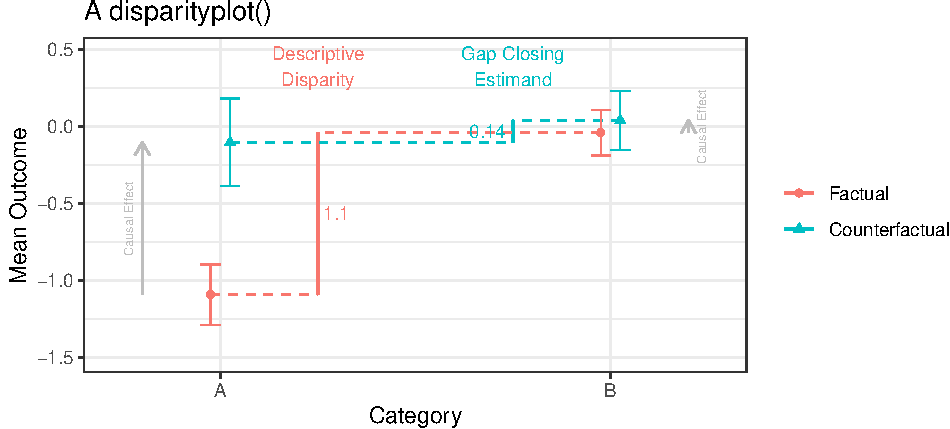
\includegraphics{github_doc_files/figure-latex/unnamed-chunk-13-1.pdf}

The \texttt{summary} function will print estimates, standard errors, and confidence intervals for all of these results.

\begin{Shaded}
\begin{Highlighting}[]
\FunctionTok{summary}\NormalTok{(estimate)}
\CommentTok{\#\textgreater{} Gap{-}closing estimates using doubly\_robust estimation on one sample.}
\CommentTok{\#\textgreater{} }
\CommentTok{\#\textgreater{} Treatment model was glm estimation with model formula:}
\CommentTok{\#\textgreater{} formula(treatment \textasciitilde{} confounder + category)}
\CommentTok{\#\textgreater{} }
\CommentTok{\#\textgreater{} Outcome model was lm estimation with model formula:}
\CommentTok{\#\textgreater{} formula(outcome \textasciitilde{} confounder + category * treatment)}
\CommentTok{\#\textgreater{} }
\CommentTok{\#\textgreater{} Factual estimates are means within and disparities across category.}
\CommentTok{\#\textgreater{} Counterfactual estimates are under an intervention to set  to 1.}
\CommentTok{\#\textgreater{} Standard errors are calculated from 20 bootstrap samples.}
\CommentTok{\#\textgreater{} }
\CommentTok{\#\textgreater{} Factual mean outcomes:}
\CommentTok{\#\textgreater{} \# A tibble: 3 x 5}
\CommentTok{\#\textgreater{}   category estimate     se ci.min ci.max}
\CommentTok{\#\textgreater{}   \textless{}chr\textgreater{}       \textless{}dbl\textgreater{}  \textless{}dbl\textgreater{}  \textless{}dbl\textgreater{}  \textless{}dbl\textgreater{}}
\CommentTok{\#\textgreater{} 1 A         {-}1.09   0.100  {-}1.29  {-}0.894}
\CommentTok{\#\textgreater{} 2 B         {-}0.0384 0.0759 {-}0.187  0.110}
\CommentTok{\#\textgreater{} 3 C          0.495  0.0833  0.332  0.659}
\CommentTok{\#\textgreater{} }
\CommentTok{\#\textgreater{} Counterfactual mean outcomes (post{-}intervention means):}
\CommentTok{\#\textgreater{} \# A tibble: 3 x 5}
\CommentTok{\#\textgreater{}   category estimate     se  ci.min ci.max}
\CommentTok{\#\textgreater{}   \textless{}chr\textgreater{}       \textless{}dbl\textgreater{}  \textless{}dbl\textgreater{}   \textless{}dbl\textgreater{}  \textless{}dbl\textgreater{}}
\CommentTok{\#\textgreater{} 1 A         {-}0.102  0.145  {-}0.386   0.182}
\CommentTok{\#\textgreater{} 2 B          0.0409 0.0974 {-}0.150   0.232}
\CommentTok{\#\textgreater{} 3 C          0.0805 0.0852 {-}0.0865  0.248}
\CommentTok{\#\textgreater{} }
\CommentTok{\#\textgreater{} Factual disparities:}
\CommentTok{\#\textgreater{} \# A tibble: 6 x 5}
\CommentTok{\#\textgreater{}   category estimate    se ci.min ci.max}
\CommentTok{\#\textgreater{}   \textless{}chr\textgreater{}       \textless{}dbl\textgreater{} \textless{}dbl\textgreater{}  \textless{}dbl\textgreater{}  \textless{}dbl\textgreater{}}
\CommentTok{\#\textgreater{} 1 A {-} B      {-}1.05  0.145 {-}1.34  {-}0.768}
\CommentTok{\#\textgreater{} 2 A {-} C      {-}1.59  0.137 {-}1.85  {-}1.32 }
\CommentTok{\#\textgreater{} 3 B {-} A       1.05  0.145  0.768  1.34 }
\CommentTok{\#\textgreater{} 4 B {-} C      {-}0.534 0.103 {-}0.737 {-}0.331}
\CommentTok{\#\textgreater{} 5 C {-} A       1.59  0.137  1.32   1.85 }
\CommentTok{\#\textgreater{} 6 C {-} B       0.534 0.103  0.331  0.737}
\CommentTok{\#\textgreater{} }
\CommentTok{\#\textgreater{} Counterfactual disparities (gap{-}closing estimands):}
\CommentTok{\#\textgreater{} \# A tibble: 6 x 5}
\CommentTok{\#\textgreater{}   category estimate    se ci.min ci.max}
\CommentTok{\#\textgreater{}   \textless{}chr\textgreater{}       \textless{}dbl\textgreater{} \textless{}dbl\textgreater{}  \textless{}dbl\textgreater{}  \textless{}dbl\textgreater{}}
\CommentTok{\#\textgreater{} 1 A {-} B     {-}0.143  0.178 {-}0.491  0.205}
\CommentTok{\#\textgreater{} 2 A {-} C     {-}0.183  0.172 {-}0.520  0.155}
\CommentTok{\#\textgreater{} 3 B {-} A      0.143  0.178 {-}0.205  0.491}
\CommentTok{\#\textgreater{} 4 B {-} C     {-}0.0396 0.113 {-}0.260  0.181}
\CommentTok{\#\textgreater{} 5 C {-} A      0.183  0.172 {-}0.155  0.520}
\CommentTok{\#\textgreater{} 6 C {-} B      0.0396 0.113 {-}0.181  0.260}
\CommentTok{\#\textgreater{} }
\CommentTok{\#\textgreater{} Additive gap closed: Counterfactual {-} Factual}
\CommentTok{\#\textgreater{} \# A tibble: 6 x 5}
\CommentTok{\#\textgreater{}   category estimate     se ci.min ci.max}
\CommentTok{\#\textgreater{}   \textless{}chr\textgreater{}       \textless{}dbl\textgreater{}  \textless{}dbl\textgreater{}  \textless{}dbl\textgreater{}  \textless{}dbl\textgreater{}}
\CommentTok{\#\textgreater{} 1 A {-} B      {-}0.909 0.157  {-}1.22  {-}0.602}
\CommentTok{\#\textgreater{} 2 A {-} C      {-}1.40  0.120  {-}1.64  {-}1.17 }
\CommentTok{\#\textgreater{} 3 B {-} A       0.909 0.157   0.602  1.22 }
\CommentTok{\#\textgreater{} 4 B {-} C      {-}0.494 0.0979 {-}0.686 {-}0.302}
\CommentTok{\#\textgreater{} 5 C {-} A       1.40  0.120   1.17   1.64 }
\CommentTok{\#\textgreater{} 6 C {-} B       0.494 0.0979  0.302  0.686}
\CommentTok{\#\textgreater{} }
\CommentTok{\#\textgreater{} Proportional gap closed: (Counterfactual {-} Factual) / Factual}
\CommentTok{\#\textgreater{} \# A tibble: 6 x 5}
\CommentTok{\#\textgreater{}   category estimate    se ci.min ci.max}
\CommentTok{\#\textgreater{}   \textless{}chr\textgreater{}       \textless{}dbl\textgreater{} \textless{}dbl\textgreater{}  \textless{}dbl\textgreater{}  \textless{}dbl\textgreater{}}
\CommentTok{\#\textgreater{} 1 A {-} B       0.864 0.155  0.559   1.17}
\CommentTok{\#\textgreater{} 2 A {-} C       0.885 0.102  0.685   1.09}
\CommentTok{\#\textgreater{} 3 B {-} A       0.864 0.155  0.559   1.17}
\CommentTok{\#\textgreater{} 4 B {-} C       0.926 0.198  0.537   1.31}
\CommentTok{\#\textgreater{} 5 C {-} A       0.885 0.102  0.685   1.09}
\CommentTok{\#\textgreater{} 6 C {-} B       0.926 0.198  0.537   1.31}
\CommentTok{\#\textgreater{} }
\CommentTok{\#\textgreater{} Type plot(name\_of\_this\_object) to visualize results.}
\end{Highlighting}
\end{Shaded}

\hypertarget{concepts-in-detail}{%
\section{Concepts in detail}\label{concepts-in-detail}}

This section provides a more detailed overview of the use of \texttt{gapclosing()}.

It is structured from the perspective of the three key tasks for the researcher:

\begin{enumerate}
\def\labelenumi{\arabic{enumi}.}
\tightlist
\item
  define the intervention
\item
  make causal assumptions for identification
\item
  specify a treatment and/or outcome model
\end{enumerate}

Along the way, this section introduces many of the possible arguments in a \texttt{gapclosing()} call.

\hypertarget{define-the-intervention}{%
\subsection{Define the intervention}\label{define-the-intervention}}

To answer a gap-closing question, we first need to define what that intervention would be. To what treatment value would units be counterfactually assigned? There are several options.

\begin{itemize}
\tightlist
\item
  \textbf{Option 1.} Set \texttt{counterfactual\_assignments\ =\ 0} or \texttt{counterfactual\_assignments\ =\ 1}. In this case, we are studying the disparity we would expect if a random person of each category were assigned control or if assigned treatment (respectively).
\item
  \textbf{Option 2.} Set \texttt{counterfactual\_assignments} = \(\pi\) for some \(\pi\) between 0 and 1. In this case, we are studying the disparity we would expect if a random person of each category were assigned to treatment with probability \(\pi\) and to control with probability \(1 - \pi\).
\item
  \textbf{Option 3.} Assign treatments by a probability \(\pi_i\) that may differ for each person \(i\). In this case, we create a vector \(\vec\pi\) of length \(n\) and pass that in the \texttt{counterfactual\_assignments} argument.
\end{itemize}

\begin{quote}
\emph{Example.} We are interested in the disparity across populations defined by \texttt{category} that would persist under counterfactual assignment to set \texttt{treatment} to the value 1.
\texttt{counterfactual\_assignments\ =\ 1}
\end{quote}

\hypertarget{make-causal-assumptions-for-identification}{%
\subsection{Make causal assumptions for identification}\label{make-causal-assumptions-for-identification}}

The package does help you with this step. Gap-closing estimands involve unobserved potential outcomes. Because they are unobserved, the data cannot tell us which variables are needed for estimation. Instead, that is a conceptual choice to be carried out with tools like Directed Acyclic Graphs (DAGs). See the accompanying \citet{lundberg2021} paper for more on identification.

\begin{quote}
\emph{Example.} Assume that the set of variables \(\{X,L\}\) is a sufficient conditioning set to identify the gap-closing estimand. Formally, this requires us to assume that within each stratum of \(X\) and \(L\) the expected value of the potential outcome \(Y(1)\) is the same as the expected value among units who factually have \(T = 1\) within those strata.
\[\mathbb{E}(Y(1)\mid X, L) = \mathbb{E}(Y\mid X, L, T = 1)\]
DAGs are a good way to reason about this assumption: in this example, conditioning (depicted by boxes) on \texttt{category} and \texttt{confounder} is sufficient to identify the causal effect of \texttt{treatment} (blue edge in the DAG), because doing so blocks all backdoor paths between the treatment and the outcome. Notably, the gap-closing estimand makes no claims about the causal effect of \texttt{category} since the counterfactual is defined over \texttt{treatment} only.
\end{quote}

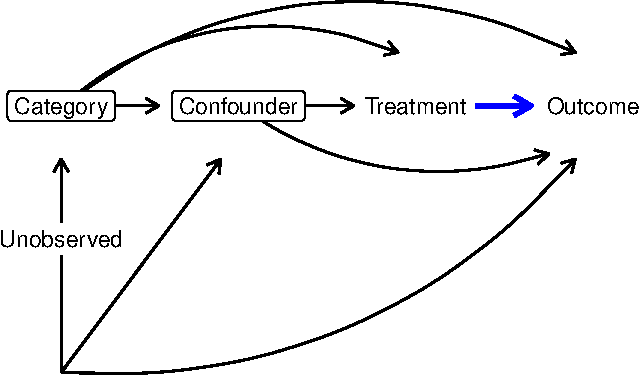
\includegraphics{github_doc_files/figure-latex/unnamed-chunk-18-1.pdf}

Once we select a sufficient conditioning set, those predictors will appear in both the treatment and/or the outcome model used for estimation.

\hypertarget{specify-a-treatment-model-andor-an-outcome-model}{%
\subsection{Specify a treatment model and/or an outcome model}\label{specify-a-treatment-model-andor-an-outcome-model}}

We need to estimate one or both of (1) the probability of treatment given confounders and (2) the conditional mean of the outcome given treatment and confounders. We do that by providing one or both of the following.

\begin{itemize}
\tightlist
\item
  Provide a \texttt{treatment\_formula} with the binary treatment variable on the left side and all confounders on the right side. This formula will be used in \texttt{treatment\_algorithm} (see next step) to estimate the probability of treatment given confounders for each unit. Then, the sample-average outcome under counterfactual assignment to any given treatment can be estimated through inverse probability weighting among units who factually received that treatment.
\end{itemize}

\begin{quote}
\emph{Example.}\\
\texttt{treatment\_formula\ =\ formula(outcome\ \textasciitilde{}\ confounder\ +\ category)}
\end{quote}

\begin{itemize}
\tightlist
\item
  Provide an \texttt{outcome\_formula} with the outcome variable on the left side and the treatment and all confounders on the right side. This formula will be used in \texttt{outcome\_algorithm} (see next step) to estimate the conditional mean of the outcome given treatment and confounders. Then, it can be used to predict the potential outcome each unit would expect under any treatment of interest, given confounding variables.
\end{itemize}

\begin{quote}
\emph{Example.}\\
\texttt{outcome\_formula\ =\ formula(outcome\ \textasciitilde{}\ confounder\ +\ category*treatment)}
\end{quote}

Whether \texttt{treatment\_formula} or \texttt{outcome\_formula} is left \texttt{NULL} will determine the estimation procedure.

\begin{itemize}
\tightlist
\item
  If only \texttt{treatment\_formula} is provided, then estimation will be by inverse probability of treatment weighting.
\item
  If only \texttt{outcome\_formula} is provided, then estimation will be by prediction of unobserved potential outcomes (the \(g\)-formula, see \citet{hernan2021}).
\item
  If both \texttt{treatment\_formula} and \texttt{outcome\_formula} are provided, then the primary estimate will be doubly robust, with separate treatment and outcome modeling estimates accessible through the returned object.
\end{itemize}

\hypertarget{choose-an-estimation-algorithm}{%
\subsubsection{Choose an estimation algorithm}\label{choose-an-estimation-algorithm}}

The \texttt{treatment\_formula} and \texttt{outcome\_formula} are handed to \texttt{treatment\_algorithm} and \texttt{outcome\_algorithm}, which can take the following values.

\begin{itemize}
\tightlist
\item
  \texttt{glm} (for \texttt{treatment\_algorithm} only): A logistic regression model estimated by the \texttt{glm} function. If there are important interactions among treatment, category, and covariates, these should be included explicitly.
\item
  \texttt{lm} (for \texttt{outcome\_algorithm} only): An OLS regression model estimated by the \texttt{lm} function. If there are important interactions among treatment, category, and covariates, these should be included explicitly.
\item
  \texttt{ridge}: A ridge (i.e.~L2-penalized) logistic regression model (for \texttt{treatment\_algorithm}) or linear regression model (for \texttt{outcome\_algorithm}) estimated by the \texttt{glmnet} function in the \texttt{glmnet} package \citep{glmnet}, with \texttt{alpha\ =\ 0} to indicate the ridge penalty. Elastic net and lasso regression are not supported because those approaches could regularize some coefficients to exactly zero, and if you have chosen the needed confounders (step 2) then you would not want their coefficients to be regularized to zero. The penalty term is chosen by \texttt{cv.glmnet} and is set to the value \texttt{lambda.min} (see \texttt{glmnet} documentation). If there are important interactions among treatment, category, and covariates, these should be included explicitly.
\item
  \texttt{gam}: A Generalized Additive Model (logistic if used as \texttt{treatment\_algorithm}, linear if used as \texttt{outcome\_algorithm}) estimated by the \texttt{gam} function in the \texttt{mgcv} package \citep{mgcv}. The model formula should be specified as in the \texttt{mgcv} documentation and may include smooth terms \texttt{s()} for continuous covariates. If there are important interactions among treatment, category, and covariates, these should be included explicitly.
\item
  \texttt{ranger}: A random forest estimated by the \texttt{ranger} function in the \texttt{ranger} package \citep{ranger}. If used as \texttt{treatment\_algorithm}, one forest will be fit and predicted treatment probabilities will be truncated to the {[}.001,.999{]} range to avoid extreme inverse probability of treatment weights. If used as \texttt{outcome\_algorithm}, the forest will be estimated separately on treated and control units; the treatment variable does not need to be included in \texttt{outcome\_formula} in this case.
\end{itemize}

\begin{quote}
\emph{Example.}\\
\texttt{treatment\_algorithm\ =\ "glm"}\strut \\
\texttt{outcome\_algorithm\ =\ "lm"}
\end{quote}

If the data are a sample from a population selected with unequal probabilities, you can also use the \texttt{weight\_name} option to pass estimation functions the name of the sampling weight (a variable in \texttt{data} proportional to the inverse probability of sample inclusion). If omitted, a simple random sample is assumed.

\hypertarget{why-doubly-robust-a-side-note}{%
\subsubsection{Why doubly robust? A side note}\label{why-doubly-robust-a-side-note}}

Doubly-robust estimation yields advantages that can be conceptualized in two ways.

\begin{itemize}
\tightlist
\item
  From the perspective of parametric models, if either the treatment or the outcome model is correct, then the estimator is consistent \citep{bang2005}. See \citet{glynn2010} for an accessible introduction.\\
\item
  From the perspective of machine learning, double robustness adjusts for the fact that outcome modeling alone is optimized for the wrong prediction task. An outcome model would be optimized to predict where we observed data, but our actual task is to predict over a predictor distribution \emph{different} from that which was observed (because the treatment has been changed). This is an opportunity to improve the predictions. By building a model of treatment, we can reweight the residuals of the outcome model to estimate the average prediction error over the space where we want to make predictions. Subtracting off this bias can improve the outcome modeling estimator. This pivot is at the core of moves toward targeted learning \citep{vanderlaan2011} and double machine learning \citep{chernozhukov2018}, building on a long line of research in efficient estimation \citep{robins1995, hahn1998}.
\end{itemize}

Although double robustness has strong mathematical properties, in any given application with a finite sample it is possible that treatment or outcome modeling could outperform doubly-robust estimation. Therefore, the package supports all three approaches.

\hypertarget{why-sample-splitting-another-side-note}{%
\subsubsection{Why sample splitting? Another side note}\label{why-sample-splitting-another-side-note}}

Taking the bias-correction view of double robustness above, it is clear that sample splitting affords a further opportunity for improvement: if you learn an outcome model \emph{and} estimate its average bias on the same sample, you might get a poor estimate of the bias. For this reason, one should consider using one sample (which I call \texttt{data\_learn}) to learn the prediction functions and another sample (which I call \texttt{data\_estimate}) to estimate the bias and aggregate to an estimate of the estimand.

In particular, the option \texttt{sample\_split\ =\ "cross\_fit"} allows the user to specify that estimation should proceed by a cross-fitting procedure which is analogous to cross-validation.

\begin{enumerate}
\def\labelenumi{\arabic{enumi}.}
\tightlist
\item
  Split the sample into folds \(f = 1,\dots,\)\texttt{n\_folds} (default here is \texttt{n\_folds\ =\ 2})\\
\item
  Use all folds except \(f'\) to estimate the treatment and outcome models\\
\item
  Aggregate to an estimate using the predictions in \(f'\)\\
\item
  Average the estimate that results from (2) and (3) repeated \texttt{n\_folds} times with each fold playing the role of \(f'\) in turn
\end{enumerate}

This is the procedure that \citet{chernozhukov2018} argue is critical to double machine learning for causal estimation, although this type of sample splitting is not new \citep{bickel1982}.

If \texttt{sample\_split\ =\ "cross\_fit"}, the default is to conduct 2-fold cross-fitting, but this can be changed with the \texttt{n\_folds} argument. The user can also specify their own vector \texttt{folds} of fold assignments of length \texttt{nrow(data)}, if there is something about the particular setting that would make a manual fold assignment preferable.

\begin{quote}
\emph{Example.} (this is the default and can be left implicit)\\
\texttt{sample\_split\ =\ "one\_sample"}
\end{quote}

\hypertarget{produce-standard-errors}{%
\subsubsection{Produce standard errors}\label{produce-standard-errors}}

The package supports bootstrapped standard error estimation. The procedure with \texttt{bootstrap\_method\ =\ "simple"} (the default) is valid when the data are a simple random sample from the target population. In this case, each bootstrap iteration conducts estimation on a resampled dataset selected with replacement with equal probabilities. The standard error is calculated as the standard deviation of the estimate across bootstrap samples, and confidence intervals are calculated by a normal approximation.

\begin{quote}
\emph{Example.} (line 2 is the default and can be left implicit)\\
\texttt{se\ =\ T}
\texttt{bootstrap\_samples\ =\ 1000}
\end{quote}

In some settings, the sample size may be small and categories or treatments of interest may be rare. In these cases, it is possible for one or more simple bootstrap samples to contain zero cases in some (treatment \(\times\) category) cell of interest. To avoid this problem, \texttt{bootstrap\_method\ =\ "stratified"} conducts bootstrap resampling within blocks defined by (treatment \(\times\) category). This procedure is valid if you assume that the data are selected at random from the population within these strata, so that across repeated samples from the true population the proportion in each stratum would remain the same.

Many samples are not simple random samples. In complex sample settings, users should implement their own standard error procedures to accurately capture sampling variation related to how their data were collected. The way the data were collected could motivate a resampling strategy to mimic the sources of variation in that sampling process, which the user can implement manually by calling \texttt{gapclosing} to calculate a point estimate on each resampled dataset with \texttt{se\ =\ FALSE}.

\hypertarget{machine-learning-examples}{%
\section{Machine learning examples}\label{machine-learning-examples}}

Suppose you want to relax parametric functional form assumptions by plugging in a machine learning estimator. As the user, this simply involves changing the arguments to the \texttt{gapclosing()} function.

\hypertarget{generalized-additive-models}{%
\subsection{Generalized Additive Models}\label{generalized-additive-models}}

Perhaps you are concerned about linearity assumptions: the continuous confounder, for instance, might actually have a nonlinear association with the outcome. We know the truth is linear in this simulated example, but in practice you would never know. You can address this concern by estimating with a GAM, using the \texttt{s()} operator from \texttt{mgcv} for smooth terms (see \citet{mgcv}).

\begin{Shaded}
\begin{Highlighting}[]
\NormalTok{estimate\_gam }\OtherTok{\textless{}{-}} \FunctionTok{gapclosing}\NormalTok{(}
  \AttributeTok{data =}\NormalTok{ simulated\_data,}
  \AttributeTok{counterfactual\_assignments =} \DecValTok{1}\NormalTok{,}
  \AttributeTok{outcome\_formula =} \FunctionTok{formula}\NormalTok{(outcome }\SpecialCharTok{\textasciitilde{}} \FunctionTok{s}\NormalTok{(confounder) }\SpecialCharTok{+}\NormalTok{ category}\SpecialCharTok{*}\NormalTok{treatment),}
  \AttributeTok{treatment\_formula =} \FunctionTok{formula}\NormalTok{(treatment }\SpecialCharTok{\textasciitilde{}} \FunctionTok{s}\NormalTok{(confounder) }\SpecialCharTok{+}\NormalTok{ category),}
  \AttributeTok{category\_name =} \StringTok{"category"}\NormalTok{,}
  \AttributeTok{treatment\_algorithm =} \StringTok{"gam"}\NormalTok{,}
  \AttributeTok{outcome\_algorithm =} \StringTok{"gam"}\NormalTok{,}
  \AttributeTok{sample\_split =} \StringTok{"cross\_fit"}
  \CommentTok{\# Note: Standard errors with \textasciigrave{}se = TRUE\textasciigrave{} are supported.}
  \CommentTok{\# They are omitted here only to speed vignette build time.}
\NormalTok{)}
\end{Highlighting}
\end{Shaded}

\hypertarget{random-forests}{%
\subsection{Random forests}\label{random-forests}}

Perhaps you are concerned that the true treatment probability and expected outcome functions have many interactions among the predictors. You can set \texttt{treatment\_algorithm} and \texttt{outcome\_algorithm} to ``ranger'' to estimate via the \texttt{ranger} function in the \texttt{ranger} package \citep{ranger}.

One aspect of the way \texttt{gapclosing()} operationalizes \texttt{ranger()} is unique out of all the estimation algorithm options. When you choose a random forest, it is because you believe there are many important interactions. Some of the most important interactions may be between the treatment and the other predictors. Therefore, \texttt{outcome\_algorithm\ =\ ranger} enforces those interactions by estimating the outcome model separately for treated and control units. For this reason, when \texttt{outcome\_algorithm\ =\ ranger} there is no need to include the treatment variable explicitly in the \texttt{outcome\_formula}.

\begin{Shaded}
\begin{Highlighting}[]
\NormalTok{estimate\_ranger }\OtherTok{\textless{}{-}} \FunctionTok{gapclosing}\NormalTok{(}
  \AttributeTok{data =}\NormalTok{ simulated\_data,}
  \AttributeTok{counterfactual\_assignments =} \DecValTok{1}\NormalTok{,}
  \AttributeTok{outcome\_formula =} \FunctionTok{formula}\NormalTok{(outcome }\SpecialCharTok{\textasciitilde{}}\NormalTok{ confounder }\SpecialCharTok{+}\NormalTok{ category),}
  \AttributeTok{treatment\_formula =} \FunctionTok{formula}\NormalTok{(treatment }\SpecialCharTok{\textasciitilde{}}\NormalTok{ confounder }\SpecialCharTok{+}\NormalTok{ category),}
  \AttributeTok{category\_name =} \StringTok{"category"}\NormalTok{,}
  \AttributeTok{treatment\_algorithm =} \StringTok{"ranger"}\NormalTok{,}
  \AttributeTok{outcome\_algorithm =} \StringTok{"ranger"}\NormalTok{,}
  \AttributeTok{sample\_split =} \StringTok{"cross\_fit"}
  \CommentTok{\# Note: Standard errors with \textasciigrave{}se = TRUE\textasciigrave{} are supported.}
  \CommentTok{\# They are omitted here only to speed vignette build time.}
\NormalTok{)}
\end{Highlighting}
\end{Shaded}

\hypertarget{estimates-from-these-three-algorithms-are-roughly-the-same}{%
\subsection{Estimates from these three algorithms are roughly the same}\label{estimates-from-these-three-algorithms-are-roughly-the-same}}

In this simulation, the GLM models are correctly specified and there are no nonlinearities or interactions for the machine learning approaches to learn. In this case, the sample size is large enough that those approaches correctly learn the linear functional form, and all three estimation strategies yield similar estimates.

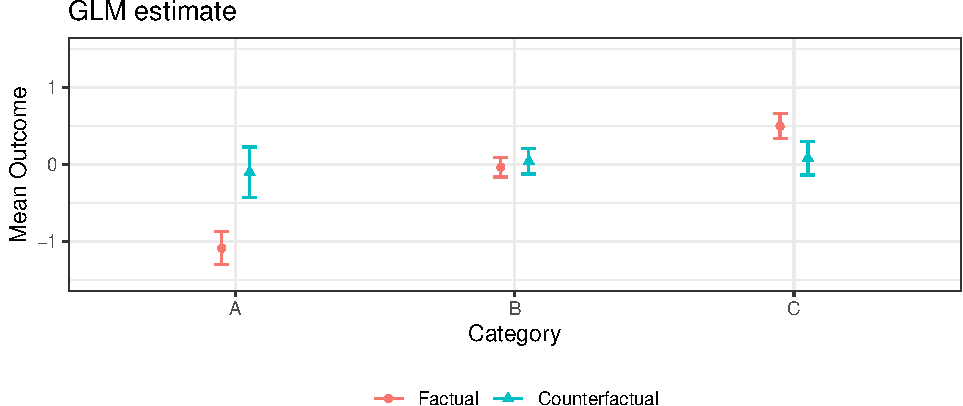
\includegraphics{github_doc_files/figure-latex/unnamed-chunk-23-1.pdf} 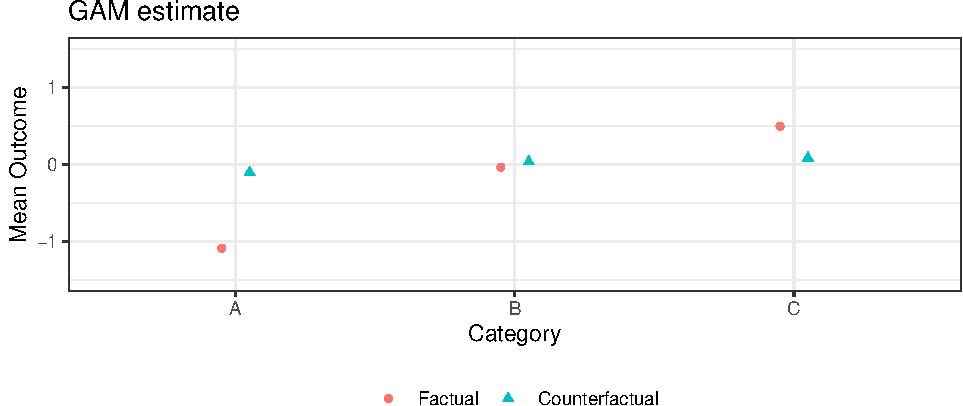
\includegraphics{github_doc_files/figure-latex/unnamed-chunk-23-2.pdf} 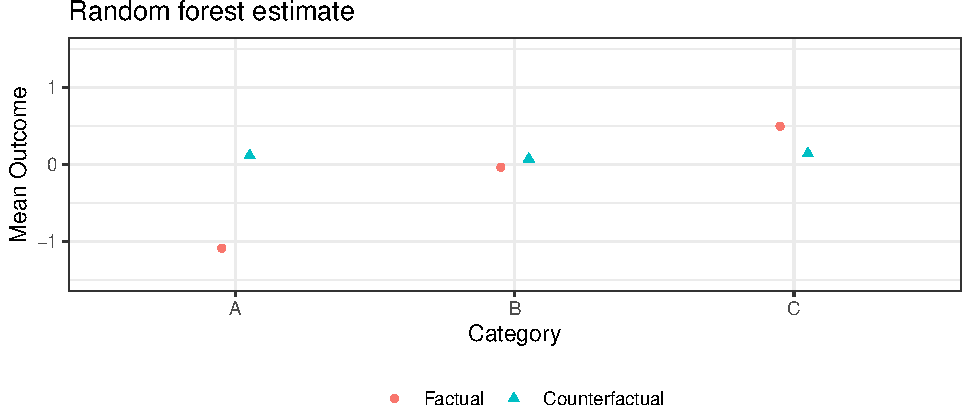
\includegraphics{github_doc_files/figure-latex/unnamed-chunk-23-3.pdf}

Note that confidence intervals for GAM and random forest can also be generated with \texttt{SE\ =\ TRUE}, which is turned off here only to speed vignette build time.

\hypertarget{word-of-warning}{%
\subsection{Word of warning}\label{word-of-warning}}

The assumptions of a parametric model are always doubtful, leading to a common question of whether one should always use a more flexible machine learning approach like \texttt{ranger}. In a very large sample, a flexible learner would likely be the correct choice. In the sample sizes of social science settings, the amount of data may sometimes be insufficient for these algorithms to discover a complex functional form. When the parametric assumptions are approximately true, the parametric estimators may have better performance in small sample sizes. What counts as ``small'' and ``large'' is difficult to say outside of any specific setting.

\hypertarget{advanced-treatment-assignments}{%
\section{Advanced treatment assignments}\label{advanced-treatment-assignments}}

So far, we have focused on estimation for a fixed treatment assignment: assign to treatment 1 with probability 1.

We might also want to know about the gap-closing estimand

\begin{itemize}
\tightlist
\item
  if we assigned people to treatment stochastically
\item
  if each person's assignment were individualized
\end{itemize}

\hypertarget{stochastic-treatments}{%
\subsection{Stochastic treatments}\label{stochastic-treatments}}

We may want to study a counterfactual where treatment is assigned with some probability between 0 and 1. The \texttt{counterfactual\_assignments} argument can handle this possibility.

For example, consider the gap-closing estimand if assigned to treatment 1 with each probability .75.

\begin{Shaded}
\begin{Highlighting}[]
\NormalTok{estimate\_stochastic }\OtherTok{\textless{}{-}} \FunctionTok{gapclosing}\NormalTok{(}
  \AttributeTok{data =}\NormalTok{ simulated\_data,}
  \AttributeTok{counterfactual\_assignments =}\NormalTok{ .}\DecValTok{75}\NormalTok{,}
  \AttributeTok{outcome\_formula =} \FunctionTok{formula}\NormalTok{(outcome }\SpecialCharTok{\textasciitilde{}}\NormalTok{ confounder }\SpecialCharTok{+}\NormalTok{ category}\SpecialCharTok{*}\NormalTok{treatment),}
  \AttributeTok{treatment\_formula =} \FunctionTok{formula}\NormalTok{(treatment }\SpecialCharTok{\textasciitilde{}}\NormalTok{ confounder }\SpecialCharTok{+}\NormalTok{ category),}
  \AttributeTok{category\_name =} \StringTok{"category"}
\NormalTok{)}
\end{Highlighting}
\end{Shaded}

The disparity between categories A and B under that stochastic intervention (0.75 probability of treatment = 1) is estimated to be 0.44, whereas under the previous deterministic intervention to assign treatment to the value 1 the disparity would be 0.14. This illustrates an important point: the gap-closing estimand can be different depending on the counterfactual assignment rule, as the figure below shows for counterfactuals in which treatment is assigned with probabilities ranging from 0 to 1.
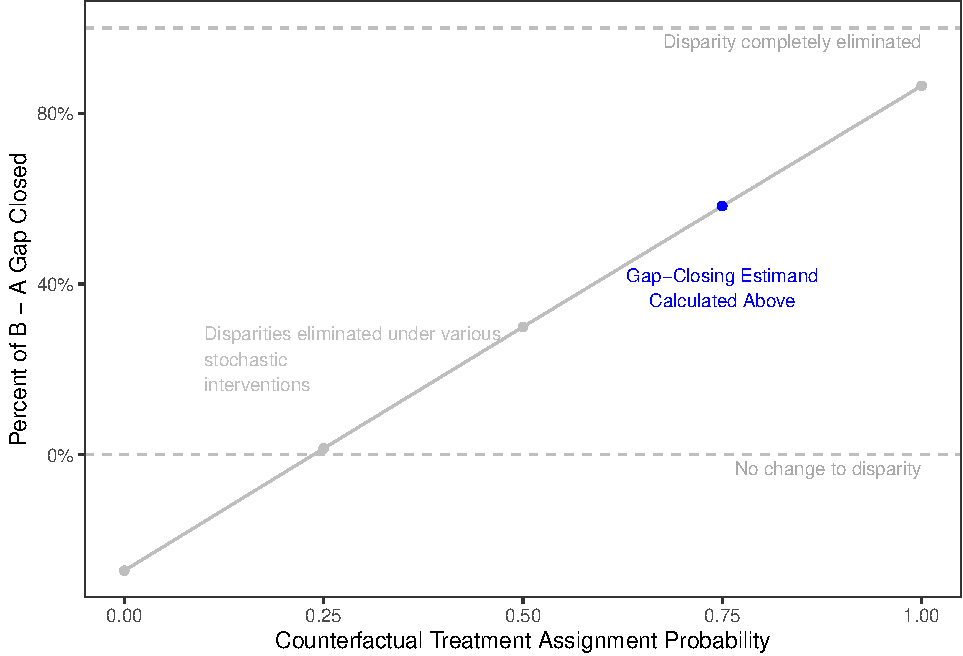
\includegraphics{github_doc_files/figure-latex/unnamed-chunk-26-1.pdf}

\hypertarget{individualized-treatments}{%
\subsection{Individualized treatments}\label{individualized-treatments}}

Treatment may also be different (and possibly stochastic) for each unit in the counterfactual world of interest.

For example, suppose we assign those in Category A to treatment 1 with probability .5, those in Category B to treatment with probability .4, and those in Category C to treatment with probability .3. In this case, \texttt{counterfactual\_assignments} will be set to a vector of length \texttt{nrow(data)}.

\begin{Shaded}
\begin{Highlighting}[]
\NormalTok{our\_assignments }\OtherTok{\textless{}{-}} \FunctionTok{case\_when}\NormalTok{(simulated\_data}\SpecialCharTok{$}\NormalTok{category }\SpecialCharTok{==} \StringTok{"A"} \SpecialCharTok{\textasciitilde{}}\NormalTok{ .}\DecValTok{5}\NormalTok{,}
\NormalTok{                             simulated\_data}\SpecialCharTok{$}\NormalTok{category }\SpecialCharTok{==} \StringTok{"B"} \SpecialCharTok{\textasciitilde{}}\NormalTok{ .}\DecValTok{4}\NormalTok{, }
\NormalTok{                             simulated\_data}\SpecialCharTok{$}\NormalTok{category }\SpecialCharTok{==} \StringTok{"C"} \SpecialCharTok{\textasciitilde{}}\NormalTok{ .}\DecValTok{3}\NormalTok{)}
\NormalTok{estimate\_stochastic }\OtherTok{\textless{}{-}} \FunctionTok{gapclosing}\NormalTok{(}
  \AttributeTok{data =}\NormalTok{ simulated\_data,}
  \AttributeTok{counterfactual\_assignments =}\NormalTok{ our\_assignments,}
  \AttributeTok{outcome\_formula =} \FunctionTok{formula}\NormalTok{(outcome }\SpecialCharTok{\textasciitilde{}}\NormalTok{ confounder }\SpecialCharTok{+}\NormalTok{ category}\SpecialCharTok{*}\NormalTok{treatment),}
  \AttributeTok{treatment\_formula =} \FunctionTok{formula}\NormalTok{(treatment }\SpecialCharTok{\textasciitilde{}}\NormalTok{ confounder }\SpecialCharTok{+}\NormalTok{ category),}
  \AttributeTok{category\_name =} \StringTok{"category"}
\NormalTok{)}
\end{Highlighting}
\end{Shaded}

That intervention would close the B - A gap by 31\%.

\hypertarget{conclusion}{%
\section{Conclusion}\label{conclusion}}

The \texttt{gapclosing} package is designed to support inquiry into gap closing estimands, thus promoting new understanding about interventions that can close gaps across social categories. The goal of the package is to automate technical tasks (sample splitting, aggregation to doubly robust estimates, visualization), thus freeing the researcher to devote more attention to scientific tasks like defining the intervention and making causal assumptions.

If you use this package and find a bug, it would be most helpful if you would create an issue on \href{https://github.com/ilundberg/gapclosing}{GitHub}. Suggestions for additional features are also welcome.

This vignette was compiled on 2023-03-08 21:51:50.

\hypertarget{computing-environment}{%
\subsection{Computing environment}\label{computing-environment}}

\begin{Shaded}
\begin{Highlighting}[]
\FunctionTok{sessionInfo}\NormalTok{()}
\CommentTok{\#\textgreater{} R version 4.2.2 (2022{-}10{-}31)}
\CommentTok{\#\textgreater{} Platform: aarch64{-}apple{-}darwin20 (64{-}bit)}
\CommentTok{\#\textgreater{} Running under: macOS Ventura 13.2.1}
\CommentTok{\#\textgreater{} }
\CommentTok{\#\textgreater{} Matrix products: default}
\CommentTok{\#\textgreater{} BLAS:   /Library/Frameworks/R.framework/Versions/4.2{-}arm64/Resources/lib/libRblas.0.dylib}
\CommentTok{\#\textgreater{} LAPACK: /Library/Frameworks/R.framework/Versions/4.2{-}arm64/Resources/lib/libRlapack.dylib}
\CommentTok{\#\textgreater{} }
\CommentTok{\#\textgreater{} locale:}
\CommentTok{\#\textgreater{} [1] en\_US.UTF{-}8/en\_US.UTF{-}8/en\_US.UTF{-}8/C/en\_US.UTF{-}8/en\_US.UTF{-}8}
\CommentTok{\#\textgreater{} }
\CommentTok{\#\textgreater{} attached base packages:}
\CommentTok{\#\textgreater{} [1] stats     graphics  grDevices utils     datasets }
\CommentTok{\#\textgreater{} [6] methods   base     }
\CommentTok{\#\textgreater{} }
\CommentTok{\#\textgreater{} other attached packages:}
\CommentTok{\#\textgreater{} [1] ggplot2\_3.4.0    dplyr\_1.1.0      gapclosing\_1.0.2}
\CommentTok{\#\textgreater{} }
\CommentTok{\#\textgreater{} loaded via a namespace (and not attached):}
\CommentTok{\#\textgreater{}  [1] Rcpp\_1.0.10       highr\_0.10        pillar\_1.8.1     }
\CommentTok{\#\textgreater{}  [4] compiler\_4.2.2    forcats\_1.0.0     iterators\_1.0.14 }
\CommentTok{\#\textgreater{}  [7] tools\_4.2.2       digest\_0.6.31     lattice\_0.20{-}45  }
\CommentTok{\#\textgreater{} [10] nlme\_3.1{-}162      evaluate\_0.20     lifecycle\_1.0.3  }
\CommentTok{\#\textgreater{} [13] tibble\_3.1.8      gtable\_0.3.1      mgcv\_1.8{-}41      }
\CommentTok{\#\textgreater{} [16] pkgconfig\_2.0.3   rlang\_1.0.6       Matrix\_1.5{-}3     }
\CommentTok{\#\textgreater{} [19] foreach\_1.5.2     cli\_3.6.0         rstudioapi\_0.14  }
\CommentTok{\#\textgreater{} [22] yaml\_2.3.7        parallel\_4.2.2    xfun\_0.37        }
\CommentTok{\#\textgreater{} [25] fastmap\_1.1.0     ranger\_0.14.1     withr\_2.5.0      }
\CommentTok{\#\textgreater{} [28] knitr\_1.42        generics\_0.1.3    vctrs\_0.5.2      }
\CommentTok{\#\textgreater{} [31] grid\_4.2.2        tidyselect\_1.2.0  glue\_1.6.2       }
\CommentTok{\#\textgreater{} [34] R6\_2.5.1          fansi\_1.0.4       rmarkdown\_2.20   }
\CommentTok{\#\textgreater{} [37] bookdown\_0.33     farver\_2.1.1      tidyr\_1.3.0      }
\CommentTok{\#\textgreater{} [40] purrr\_1.0.1       magrittr\_2.0.3    splines\_4.2.2    }
\CommentTok{\#\textgreater{} [43] scales\_1.2.1      codetools\_0.2{-}19  htmltools\_0.5.4  }
\CommentTok{\#\textgreater{} [46] colorspace\_2.1{-}0  labeling\_0.4.2    utf8\_1.2.3       }
\CommentTok{\#\textgreater{} [49] munsell\_0.5.0     doParallel\_1.0.17}
\end{Highlighting}
\end{Shaded}


  \bibliography{gapclosing.bib}

\end{document}
